% Arithmetic criteria for domino tatami tilings of rectangles
% (initially submitted as "Rectangular domino tatami tiling is in P")
\documentclass[11pt, reqno]{amsart}

% Core Packages
\usepackage{amsmath,amsfonts,amssymb,amsthm}
\usepackage{graphicx}
\usepackage{tikz}
\usepackage{xurl}
\usepackage{needspace}
\usepackage{hyperref}
\hypersetup{colorlinks=true, linkcolor=blue, citecolor=blue, urlcolor=blue}

% Standard Mathematical Theorem Environments
\newtheorem{theorem}{Theorem}[section]
\newtheorem{lemma}[theorem]{Lemma}
\newtheorem{corollary}[theorem]{Corollary}
\newtheorem{proposition}[theorem]{Proposition}

\theoremstyle{definition}
\newtheorem{definition}[theorem]{Definition}
\newtheorem{example}[theorem]{Example}

\theoremstyle{remark}
\newtheorem{remark}[theorem]{Remark}

\numberwithin{equation}{section}

\title{Arithmetic criteria for domino tatami tilings of rectangles}

\author{Rifki Kusmana}
\address{Computer Science Department\\School of Computer Science\\Bina Nusantara University\\11480\\Jakarta, Indonesia}
\email{rifki.kusmana@binus.ac.id}

\author{Alexander Agung Santoso Gunawan}
\address{Computer Science Department\\School of Computer Science\\Bina Nusantara University\\11530\\Jakarta, Indonesia}
\email{aagung@binus.edu}

\begin{document}
\begin{abstract}
    A domino tiling is \emph{tatami} when no four tiles meet at a point.
    We give arithmetic tests for whether an $r\times c$ rectangle admits
    such a tiling. Hickerson's decomposition, as developed by
    Ruskey and Woodcock, reduces the question to whether an interval of
    admissible block counts contains an integer. The tests treat odd
    and even heights separately. Using a constant number of integer
    operations, the tests determine whether the known counting formulas
    give a nonzero count.
    For binary input of length $B=\Theta(\log(r+1)+\log(c+1))$, the test
    can be evaluated in $O(B^2)$ bit operations and $O(B)$ workspace.
    The proofs specify a tiling
    through an $O(B)$-bit description of its block sequence.
    We cross-check the test against published tables and an independent
    enumerator based on perfect matchings of the grid graph.
    We also consider tatami tilings that allow monomers, and count the
    boundary monomers in the horizontal and vertical running bonds
    (brick-like patterns of offset rows or columns). Choosing the
    orientation with fewer monomers yields a tatami tiling with at most
    $\min(r,c)$ monomers, and we verify the resulting layouts computationally.
\end{abstract}

\keywords{tatami tiling, domino tiling, combinatorics, computational complexity,
    polynomial-time algorithm, monomer-dimer tiling}

\maketitle

\section{Introduction}

A domino is a $1\times2$ or $2\times1$ rectangle made of two unit
squares that share an edge. A domino tiling covers a grid region with
dominoes so that every unit square belongs to exactly one tile.
The tiles leave no gaps and do not overlap. A domino tiling is
\emph{tatami} when no four tiles meet at a point.
Figure~\ref{fig:domino-tatami} illustrates this extra restriction on
two tilings of the same rectangle.

\begin{figure}[htbp]
    \centering
    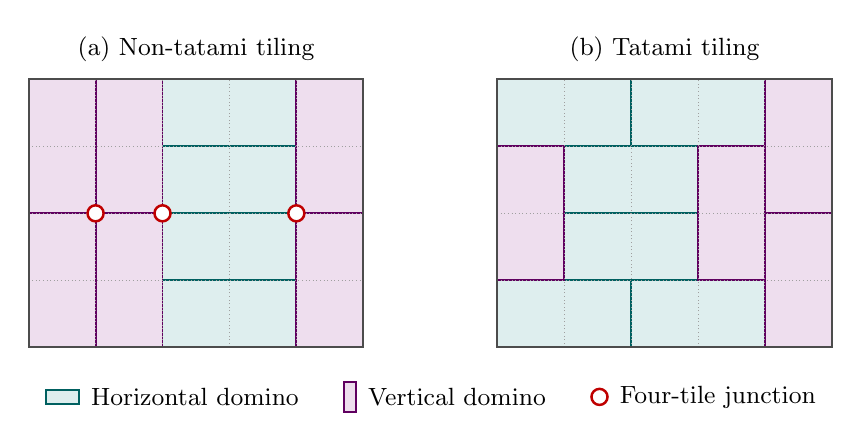
\begin{tikzpicture}[
            x=0.85cm, y=0.85cm, font=\small,
            horizontal domino/.style={draw=teal!75!black, fill=teal!13, line width=0.7pt},
            vertical domino/.style={draw=violet!75!black, fill=violet!13, line width=0.7pt},
            junction/.style={draw=red!75!black, fill=white, line width=0.9pt}
        ]
        \begin{scope}
            \node at (2.5,4.45) {(a) Non-tatami tiling};
            \foreach \x/\y in {2/0,2/1,2/2,2/3}
            \draw[horizontal domino] (\x,\y) rectangle ++(2,1);
            \foreach \x/\y in {0/0,1/0,4/0,0/2,1/2,4/2}
            \draw[vertical domino] (\x,\y) rectangle ++(1,2);
            \draw[step=1, draw=gray!75, densely dotted, line width=0.3pt]
            (0,0) grid (5,4);
            \draw[draw=black!70, line width=0.7pt] (0,0) rectangle (5,4);
            \foreach \x in {1,2,4}
            \draw[junction] (\x,2) circle[radius=0.12];
        \end{scope}
        \begin{scope}[shift={(7,0)}]
            \node at (2.5,4.45) {(b) Tatami tiling};
            \foreach \x/\y in {0/0,2/0,1/1,1/2,0/3,2/3}
            \draw[horizontal domino] (\x,\y) rectangle ++(2,1);
            \foreach \x/\y in {4/0,0/1,3/1,4/2}
            \draw[vertical domino] (\x,\y) rectangle ++(1,2);
            \draw[step=1, draw=gray!75, densely dotted, line width=0.3pt]
            (0,0) grid (5,4);
            \draw[draw=black!70, line width=0.7pt] (0,0) rectangle (5,4);
        \end{scope}
        \matrix[anchor=north, inner sep=0pt, column sep=4pt,
            nodes={inner sep=0pt, anchor=center}] at (6,-0.5) {
            \draw[horizontal domino] (-0.25,-0.1) rectangle (0.25,0.1); &
            \node {Horizontal domino};                                  & [12pt]
            \draw[vertical domino] (-0.09,-0.22) rectangle (0.09,0.22); &
            \node {Vertical domino};                                    & [12pt]
            \draw[junction] (0,0) circle[radius=0.12];                  &
            \node {Four-tile junction};                                          \\
        };
    \end{tikzpicture}
    \caption{Two domino tilings of the same $4\times5$ rectangle.
        Dotted lines mark the unit-cell boundaries. In (a), red circles
        mark the three interior points where four tiles meet. The tiling
        in (b) satisfies the tatami condition at every interior point.}
    \label{fig:domino-tatami}
\end{figure}

The \emph{Domino Tatami Covering} (DTC) problem asks whether a grid region
admits such a tiling. Erickson and Ruskey proved that DTC is NP-complete
by a reduction from planar 3SAT \cite{er13}. Their construction uses
regions with holes. The complexity for simply connected regions remains
unsettled, and they conjectured NP-completeness for that class.

For rectangles, Hickerson's block decomposition gives a description of
the possible tilings. In 2002, he gave recurrences for restricted
compositions and programs for enumerating the tilings \cite{hickerson}.
Ruskey and Woodcock proved the structural results and derived generating
functions and binomial-sum formulas for the counts
\cite[Corollary~3.4 and Theorem~3.5]{ruskey}. Evaluating the recurrences
or finding a nonzero term in those sums already decides whether a
rectangle admits a tiling.

We use this decomposition to give arithmetic tests for odd and even
heights. Each test bounds the number of blocks in a tiling. After
checking area parity, the question reduces to whether an interval of
admissible block counts contains an integer.
Lemmas~\ref{lem:odd-criterion} and~\ref{lem:even-criterion} derive these
intervals. The tests determine whether the known counting formulas give
a nonzero count without computing the counts themselves.

The interval tests require a constant number of integer operations.
For dimensions written in binary, the total input length is
$B=\Theta(\log(r+1)+\log(c+1))$. At fixed height, evaluating the
recurrence directly or scanning the counting formulas takes $\Theta(n)$
steps on the longer side $n$, which can be exponential in $B$.
Integer division computes the interval endpoints in $O(B^2)$ bit
operations with $O(B)$ workspace. The proofs in Section~\ref{sec:complexity-certificates} also specify
a tiling through an $O(B)$-bit description of its block sequence.

A rectangle admits a domino tatami tiling exactly when its minimum
number of monomers is zero. Erickson et al.\ state that T-diagrams
yield a polynomial-time method for finding this minimum
\cite[Section~4.2]{erws11}, although that passage does not include the
full algorithm or its proof. This would give another decision procedure
for the pure-domino case.

We cross-check the arithmetic tests against published tables and an
independent enumerator based on perfect matchings of the grid graph.
The enumerator does not use the block decomposition. For tilings that
allow monomers, we count the boundary monomers in the horizontal and
vertical running bonds and choose the orientation with fewer monomers.
We also verify these layouts computationally.

\Needspace{8\baselineskip}
\section{Preliminaries}
\label{sec:preliminaries}

\subsection{Problem statement and notation}
\label{sec:problem}

Let $G_{r,c}$ have one vertex for each cell of an $r\times c$ board, with
edges joining orthogonally adjacent cells. A domino tiling is a perfect
matching in this graph. The four cells around an interior grid point
form a 4-cycle. If the matching uses an edge of this cycle, two of the
cells belong to the same domino. Otherwise four distinct tiles meet at
the point. A tatami tiling is therefore a perfect matching that meets
every such cycle. Churchley, Huang, and Zhu call these matchings
\emph{$C_4$-transverse} \cite{churchley,er13}.

\begin{quote}
    \textbf{Problem RECT-DTC.} \emph{Input:} positive integers $r, c$ encoded
    in standard binary, separated by a delimiter, with total length
    $B=\Theta(\log(r+1)+\log(c+1))$.
    \emph{Question:} does the $r \times c$ grid admit a tatami domino tiling?
\end{quote}

If $rc$ is odd, no domino tiling exists. Rotation preserves domino
tilings and the tatami property. Thus, writing $T(r, c)$ for the number
of tatami tilings, we have $T(r, c) = T(c, r)$. Throughout this paper,
we let $m = \min(r, c)$ and $n = \max(r, c)$.

\emph{Encodings and computational model.} Unary dimensions
$1^r\#1^c$ have length $\Theta(r+c)$, whereas an explicit rectangular
cell array has size $\Theta(rc)$. Our main result uses binary dimensions
and counts bit operations. Reading unary dimensions or an explicit cell
array takes $\Theta(r+c)$ or $\Theta(rc)$ time, respectively.
We also describe a dynamic program whose
$O(n)$ transition bound is measured in
word-RAM operations with $O(\log n)$-bit indices. Its running time is
polynomial for unary dimensions but can be exponential in $B$.

\subsection{Structure of tatami tilings of rectangles}
\label{sec:structure}

For $m\times n$ rectangles with $m\le n$, we use the following
structural results from Hickerson's decomposition \cite{hickerson},
with the expanded proofs in \cite[Section~2]{ruskey}.

\begin{theorem}[Left-edge lemma {\cite[Theorem~2.2]{ruskey}}]
    \label{thm:left-edge}
    In a tatami tiling of an $m \times n$ rectangle with $m \le n$, no
    horizontal tile touches the left edge unless it also touches the top or
    bottom edge.
\end{theorem}

Ruskey and Woodcock prove the lemma by following the placements forced
by a horizontal tile on the left edge away from a corner. In each case,
the placements leave a staircase triangle. The coloring argument in
Remark~\ref{rem:staircase} rules out a domino tiling of that triangle.

\begin{theorem}[Odd heights {\cite[Theorem~2.3]{ruskey}}]
    \label{thm:odd}
    If $m\ge3$ is odd and $m \le n$, every tatami tiling of the $m \times n$
    rectangle is a concatenation of tiled $m \times (m-1)$ and $m \times
        (m+1)$ blocks.
\end{theorem}

\begin{theorem}[Even heights {\cite[Theorem~2.4]{ruskey}}]
    \label{thm:even}
    If $m$ is even, $m \ge 4$, and $m \le n$, every tatami tiling of the $m
        \times n$ rectangle is a strict alternation of width-1 all-vertical
    columns ($S$-blocks) and long blocks of width $m-2$ or $m$ ($L$-blocks),
    where the tiling may start and end with either type.
\end{theorem}

For $n\ge m\ge3$, an $m\times n$ rectangle has a tatami tiling if and
only if $n$ is the total width of a block sequence allowed by
Theorem~\ref{thm:odd} or~\ref{thm:even}, according to the parity of $m$.
The block templates in \cite{hickerson,ruskey} realize every such
sequence. For odd $m$, a nonempty sequence of widths $m-1$ and $m+1$
with sum $n$ gives two tilings, one for each initial seam orientation,
with subsequent seam orientations alternating. For even $m$, an alternating
sequence of $S$- and $L$-blocks with sum $n$ gives one tiling.

\begin{remark}[Staircase triangles]
    \label{rem:staircase}
    For an integer $\ell\ge1$, let $S_\ell$ be the left-aligned staircase
    region with consecutive rows of length $1, 2, \dots, \ell$.
    Color its cells as a chessboard, with the length-1 row black. Each
    even-length row has equal numbers of black and white cells. Each
    odd-length row has one extra black cell, giving a total imbalance of
    $\lceil \ell/2 \rceil \ge 1$. A domino covers one cell of each color.
    Hence $S_\ell$, and every rotation or reflection of it, admits no
    domino tiling.
\end{remark}

Heights one and two admit direct constructions.

\begin{lemma}[Small heights]
    \label{lem:small}
    A $1 \times n$ rectangle has a tatami tiling if and only if $n$ is even.
    When it exists, the tiling is unique and all dominoes are horizontal.
    A $2 \times n$ rectangle has a tatami tiling for
    every $n$, consisting of $n$ side-by-side vertical dominoes whose
    corners meet only pairwise on the boundary.
\end{lemma}

\emph{Notes on the cited proofs.} After the first block in
Theorem~\ref{thm:odd}, the seam mirrors from bottom to top. Vertical
symmetry gives the same block widths. The caption of \cite[Figure~11]{ruskey}
reads ``when $n$ is even'' where the proof requires
``$m$ is even''. The proof text itself is correct.

\section{Arithmetic criteria for tileability}
\label{sec:criteria}

\subsection{The decision procedure}
\label{sec:decision}

The procedure \texttt{DECIDE}$(r,c)$ uses the criteria proved in
Section~\ref{sec:correctness}. Set $m=\min(r,c)$ and $n=\max(r,c)$, and define
$\operatorname{ceildiv}(x,y)=\lfloor(x+y-1)/y\rfloor$ for positive
integers $x,y$. There are four cases:
\begin{enumerate}
    \item If $m = 1$, return true when $n$ is even, and false otherwise.
    \item If $m = 2$, return true for every $n$.
    \item If $m \ge 3$ is odd, return true when $n$ is even and
          $\operatorname{ceildiv}(n, m+1) \le \lfloor n / (m-1) \rfloor$.
    \item If $m \ge 4$ is even, return true when
          $\max(1, \operatorname{ceildiv}(n-1, m+1)) \le \lfloor (n+1) / (m-1) \rfloor$.
\end{enumerate}

For comparison, Hickerson's recurrences \cite{hickerson} give a dynamic
program over widths $0,\dots,n$. For odd $m\ge3$, mark width zero
reachable and extend reachable widths by $m-1$ or $m+1$. For even
$m\ge4$, keep separate states for sequences ending in an $S$-block or
an $L$-block. An $S$-state extends to an $L$-state by adding $m-2$ or
$m$, and an $L$-state extends to an $S$-state by adding 1. Initialize
the single-block sequences of widths 1, $m-2$, and $m$.

Scanning all widths takes $\Theta(n)$ word-RAM operations. The supplied
implementation stores $O(n)$ Boolean entries. Retaining only an
$(m+1)$-step window would reduce storage to $O(m)$ without changing the
time bound, but this optimization is not implemented. The arithmetic
procedure computes its answer with a constant
number of integer operations, whose bit cost is analyzed in
Section~\ref{sec:complexity-certificates}.

Pseudocode for \texttt{DECIDE} appears in
Section~\ref{sec:implementation}.

\subsection{Correctness}
\label{sec:correctness}

\begin{theorem}[Main result]
    \label{thm:main}
    RECT-DTC with binary-encoded dimensions is in P. The decision uses
    a constant number of integer operations and can be implemented in
    $O(B^2)$ bit operations with $O(B)$ workspace.
\end{theorem}

We prove correctness below and establish the complexity bounds in
Section~\ref{sec:complexity-certificates}.

For each $p\ge1$ and odd $m\ge3$, the sequences of $p$ blocks have
exactly the even widths in $[p(m-1),p(m+1)]$. For even $m\ge4$,
the alternating sequences with $p$ long blocks have exactly the
integer widths in $[p(m-1)-1,p(m+1)+1]$.

\begin{lemma}[Odd-height criterion]
    \label{lem:odd-criterion}
    For odd $m\ge3$ and $n\ge m$, an $m\times n$ rectangle is
    domino-tatami tileable if and only if $n$ is even and
    \begin{equation}
        \label{eq:odd-criterion}
        \left\lceil\frac{n}{m+1}\right\rceil
        \le
        \left\lfloor\frac{n}{m-1}\right\rfloor.
    \end{equation}
\end{lemma}

\begin{proof}
    A sequence of $p\ge1$ blocks, of which $a$ have width $m+1$,
    has total width
    \[
        n=p(m-1)+2a,\qquad 0\le a\le p.
    \]
    For fixed $p$, these are exactly the even widths from $p(m-1)$
    to $p(m+1)$. Thus a block sequence exists exactly when $n$ is even
    and there is an integer $p$ with
    $n/(m+1)\le p\le n/(m-1)$, which is
    \eqref{eq:odd-criterion}.
\end{proof}

We can also read the odd-height test from a quotient and remainder. Put
$k=(m-1)/2$ and, for even $n$, write $n/2=qk+s$ with $0\le s<k$.
The right endpoint of the block-count interval is
$\lfloor n/(m-1)\rfloor=q$. The other endpoint
satisfies $\lceil n/(m+1)\rceil\le q$ exactly when
$n/2\le q(k+1)$. Substituting the quotient and remainder reduces this
condition to $s\le q$.

\begin{lemma}[Even-height criterion]
    \label{lem:even-criterion}
    For even $m\ge4$ and $n\ge m$, an $m\times n$ rectangle is
    domino-tatami tileable if and only if
    \begin{equation}
        \label{eq:even-criterion}
        \max\left(1,\left\lceil\frac{n-1}{m+1}\right\rceil\right)
        \le
        \left\lfloor\frac{n+1}{m-1}\right\rfloor.
    \end{equation}
\end{lemma}

\begin{proof}
    Write $p$ for the number of long blocks and $b$ for the number of
    short blocks. A sequence consisting only of short blocks has width
    at most 1. Since $n\ge m\ge4$, we need $p\ge1$, and alternation
    requires $b\in\{p-1,p,p+1\}$. If $a$ long blocks have width $m$
    and the others have width $m-2$, then
    \[
        n=p(m-2)+2a+b,\qquad 0\le a\le p.
    \]
    For fixed $a$, the term $2a+b$ takes all integer values in
    $[2a+p-1,2a+p+1]$. The intervals for successive values of $a$
    share an endpoint. Their union over $0\le a\le p$ therefore
    contains every integer from $p-1$ to $3p+1$. Adding $p(m-2)$
    gives exactly the widths satisfying
    \[
        p(m-1)-1\ \le n\le\ p(m+1)+1.
    \]
    Every integer in this range has a corresponding choice of $a$ and $b$.
    The blocks can be interleaved because their numbers differ by at most
    one, and the cited seam rules give a tatami tiling. Solving the width
    bounds for an integer $p\ge1$ gives \eqref{eq:even-criterion}.
\end{proof}

Ruskey and Woodcock's binomial sums count these block choices
\cite[Corollary~3.4 and Theorem~3.5]{ruskey}. For odd $m\ge3$, a pair
of integers $(p,a)$ with $p\ge1$, $0\le a\le p$, and
$n=p(m-1)+2a$ contributes $2\binom{p}{a}$ tilings. The factor
$\binom{p}{a}$ counts the positions of the wider blocks, and the
factor 2 counts the initial seam orientations. Since every such term is
positive, $T(m,n)>0$ if and only if at least one admissible pair
exists, as characterized by Lemma~\ref{lem:odd-criterion}.

\begin{proof}[Proof of Theorem~\ref{thm:main}, correctness]
    Rotate the rectangle to place the shorter side vertically.
    Lemma~\ref{lem:small} proves the first two cases of \texttt{DECIDE}.
    Lemmas~\ref{lem:odd-criterion} and~\ref{lem:even-criterion} prove
    the other two cases, using the correspondence between tilings and
    block sequences in Section~\ref{sec:structure}.
\end{proof}

For example, at height $m=7$, every even width $n\ge7$ is tileable except
$n=10$. The allowed block widths are 6 and 8, and no sum of these widths
equals 10.

\subsection{Complexity and tiling certificates}
\label{sec:complexity-certificates}

\begin{proof}[Proof of Theorem~\ref{thm:main}, complexity]
    The procedure uses a constant number of additions, comparisons, parity
    tests, and integer divisions on $O(B)$-bit integers. Schoolbook
    division takes $O(B^2)$ bit operations and $O(B)$ workspace.
    Reading the binary input takes $O(B)$ bit operations.
    The other operations fit within these bounds, proving the theorem.
    Including the reading costs stated in Section~\ref{sec:problem}, the problem is
    also in P when dimensions are given in unary or as an explicit
    rectangular cell array.
\end{proof}

\emph{Succinct and explicit certificates.} For a yes-instance with
$m\ge3$, the parameters in the proofs of
Lemmas~\ref{lem:odd-criterion} and~\ref{lem:even-criterion} specify a
tiling. Use the
smallest admissible $p$ in each case. For odd $m$, take
\[
    p=\left\lceil\frac{n}{m+1}\right\rceil,\qquad
    a=\frac{n-p(m-1)}{2}.
\]
For even $m$, take
\[
    p=\max\left(1,\left\lceil\frac{n-1}{m+1}\right\rceil\right),\qquad
    a=\min\left(p,\left\lfloor\frac{n-p(m-1)+1}{2}\right\rfloor\right),
\]
and $b=n-p(m-2)-2a$. On a yes-instance these choices satisfy
$0\le a\le p$ and, for even $m$, $b\in\{p-1,p,p+1\}$.
Arrange the $a$ wider blocks first, followed by the $p-a$ narrower
blocks. For odd $m$, either initial seam orientation is possible, with
orientations alternating along the sequence. For even $m$, put a short
block between every pair of long blocks. When $b=p$, add one at the
end. When $b=p+1$, add one at each end.

Computing these parameters takes $O(B^2)$ bit operations, and storing
them takes $O(B)$ bits. The ordering rules and the cited block templates
\cite{hickerson,ruskey} then determine every domino. An explicit list of
domino coordinates needs $\Omega(rc)$ output entries and can be
exponentially longer than the binary input of length $B$. Expanding
the templates takes $O(rc)$ word-RAM operations. A block sequence can
also be recovered by backtracking through the dynamic program in $O(n)$
word-RAM operations. The companion implementation returns only the
decision, leaving certificate generation to these constructions.

\section{Monomer-dimer tilings and the running-bond construction}
\label{sec:running-bond}

If $1\times1$ monomers are allowed alongside dominoes, every rectangle
has a tatami tiling. One construction restricts an infinite running bond
to the rectangle and replaces dominoes cut by the boundary with monomers
\cite[Section~4]{ersw10}, \cite[Section~4.2]{erws11}.
We count the monomers for each orientation and choose the smaller count.

\Needspace{10\baselineskip}
\begin{proposition}[Running-bond construction]
    \label{prop:fallback}
    Every $r\times c$ rectangle has a monomer-dimer tatami tiling with
    $\mu=\min(\mu_H,\mu_V)\le\min(r,c)$ monomers, all on the boundary,
    where
    \begin{equation}
        \label{eq:bondcounts}
        \mu_H=
        \begin{cases}
            2\lfloor r/2\rfloor & \text{if $c$ is even}, \\
            r                   & \text{if $c$ is odd},
        \end{cases}
        \qquad
        \mu_V=
        \begin{cases}
            2\lfloor c/2\rfloor & \text{if $r$ is even}, \\
            c                   & \text{if $r$ is odd}.
        \end{cases}
    \end{equation}
    The tiling can be constructed in $O(rc)$ word-RAM operations.
\end{proposition}

\begin{proof}
    Index rows and columns from zero. In even rows of the infinite
    horizontal running bond, pair columns $(2j,2j+1)$, and in odd rows,
    pair $(2j+1,2j+2)$. Restrict this layout to the rectangle and
    replace each cell whose partner is outside by a monomer.
    At every interior grid point, exactly one of the two incident
    rows has a horizontal matched edge on its four-cell cycle.
    Both cells of that edge lie inside the rectangle, so the edge survives
    the restriction and the tiling is tatami. All cut cells lie on the boundary.

    If $c$ is even, each odd row loses its two end cells and each
    even row tiles fully. If $c$ is odd, every row loses one end cell.
    These give $\mu_H$ in \eqref{eq:bondcounts}, whereas transposition gives
    $\mu_V$. Choose the smaller count, using the horizontal orientation
    on ties. Since $\mu_H\le r$ and $\mu_V\le c$, the bound follows.
    The construction visits each cell once.
\end{proof}

Every monomer-dimer tiling has $\mu\equiv rc\pmod2$,
because the other cells occur in pairs, as noted in
\cite[Theorem~1]{erws11}. The fallback does not minimize $\mu$.
For $7\times10$, $8\times11$, and $9\times13$, it uses $6$, $8$,
and $9$ monomers, whereas direct enumeration in Section~\ref{sec:validation-results} finds
minima $2$, $2$, and $3$. Alhazov, Morita, and Iwamoto note that
$7\times10$ needs at least two monomers and $9\times13$ at least
three \cite[Section~8]{ami10}, which agrees with these minima.
Erickson et al.\ used the $9\times13$ example to show that one monomer
does not suffice for every odd-area rectangle \cite{erws11}.

\section{Computational verification}
\label{sec:computational-verification}

\subsection{Software implementation}
\label{sec:implementation}

{\tolerance=1000
    All three scripts in \mbox{\path{validation/}} use only the Python~3
    standard library. In \path{validate_tatami_dp.py}, the function
    \texttt{arithmetic\_tileable} implements \texttt{DECIDE}, and
    \texttt{tileable} evaluates the block recurrences. The script also
    counts block sequences and compares them with published tables.\par}

\Needspace{17\baselineskip}
The arithmetic function follows the pseudocode below for positive
integer inputs $r,c$. Here, \texttt{mod} denotes the remainder and
\texttt{//} denotes integer division. The function
$\operatorname{ceildiv}$ is defined in Section~\ref{sec:decision}.
\begin{verbatim}
DECIDE(r, c):
    m, n = min(r, c), max(r, c)
    if m == 1: return n mod 2 == 0
    if m == 2: return true
    if m mod 2 == 1:
        lo = ceildiv(n, m + 1)
        hi = n // (m - 1)
        return n mod 2 == 0 and lo <= hi
    lo = max(1, ceildiv(n - 1, m + 1))
    hi = (n + 1) // (m - 1)
    return lo <= hi
\end{verbatim}

An independent check comes from \mbox{\path{validate_matching_enumeration.py}}.
This script builds grid matchings one row at a time without using the
block decomposition. A profile records vertical dominoes
crossing the row boundary, horizontal dominoes placed in the preceding
row, and the current monomer count. For each new row, the script
verifies that every four-cell cycle between the two rows contains a
matched edge.

Finally, \path{validate_monomer_fallback.py} constructs and
checks the running-bond layouts described in Section~\ref{sec:running-bond}. Each script
runs from the command line, exiting with a nonzero status on failure.
Run instructions and the provenance of the comparison tables appear in
\path{validation/README.md}. The repository address is in the Data
availability statement.

\subsection{Validation results}
\label{sec:validation-results}

Direct enumeration covered 276 distinct rectangles in the union of
two ranges, $1\le m\le10$, $m\le n\le30$ and
$1\le m\le n\le16$. For every rectangle, in both input orders,
\texttt{DECIDE} and the block dynamic program returned ``yes'' exactly
when the enumerator found a tiling. The enumerator also reproduced
all 256 entries in Ruskey and Woodcock's table \cite[Table~2]{ruskey}
and all 225 in Hickerson's table \cite{hickerson}, including height two.

Both decision procedures returned ``yes'' exactly when the tabulated
count was nonzero. The block counter reproduced 227 exact
counts from Ruskey and Woodcock's table and 198 from Hickerson's.
The remaining entries have shorter side two, where the cited block
theorems do not give a counting rule. For those entries, the block
procedure only tests tileability. The direct enumerator supplies the
exact counts. The published tables share the same structural theory,
so comparisons with them serve as consistency checks.

A wider sweep compared the arithmetic criteria against the Boolean
recurrences in 162{,}752 cases, spanning $1\le m\le100$ and
$m\le n\le500$, and extending to widths as large as $10{,}000$ at
heights $m\in\{3,\allowbreak 5,\allowbreak 7,\allowbreak 8,\allowbreak
    10,\allowbreak 16,\allowbreak 31,\allowbreak 32,\allowbreak
    99,\allowbreak 100,\allowbreak 999,\allowbreak 1000\}$.
Some dimensions appear in both sweeps. Four additional tests evaluated
101-digit dimensions without allocating grid arrays.

For $7\times10$, $8\times11$, and $9\times13$, the profile enumerator
found minimum monomer counts of 2, 2, and 3, with 36, 34, and 80 tilings
at those minima. It found no tilings with fewer monomers of the
required area parity.

Running-bond verification covered all 900 rectangles with
$1\le r,c\le30$, each of the 92 domino no-instances whose dimensions
are both at most 16, and larger examples up to $1000\times999$. Every
generated layout covered each cell exactly once and obeyed the tatami
rule. Its monomer count matched the predicted count and area parity,
and every monomer lay on the boundary. These finite checks test the
implementations. The proofs establish the criteria and monomer bounds
for arbitrary dimensions.

\section{Discussion}
\label{sec:discussion}

At each fixed height, the rectangular decomposition restricts all
tilings to the stated block templates. Extending the interval argument
to other simply connected regions would require a structural description
of their tilings. Erickson and Ruskey conjectured NP-completeness for
that broader class \cite{er13}.

For a fixed height $m\ge3$, an automaton can record the block type and
seam orientation, with transitions specifying which blocks may follow.
The permitted block sequences form a regular language. Expanding each
width-$w$ block transition into a path of $w$ unit transitions gives a
unary nondeterministic finite automaton with $O(m)$ states. For
$n\ge m$, its accepted lengths are exactly the tileable widths.
The finitely many widths below $m$ can be checked separately.

For counting, give each block transition weight $z^w$ and retain the
seam orientations. The resulting transfer matrix gives Ruskey and
Woodcock's rational counting functions \cite{ruskey}. The interval
tests decide tileability without expanding the automaton or evaluating
these functions.

When the boundary is irregular, profile dynamic programming offers an
alternative, provided the region fits in a strip of fixed height~$h$.
Columns are processed one at a time. The profile records which
dominoes cross the column boundary and carries enough information from
the previous column to verify each four-cell cycle. Because both
coverage and the tatami rule depend only on these local data, the
number of distinct profiles is $2^{O(h)}$. The overall cost is
therefore $2^{O(h)}n$ word-RAM operations for a region that spans $n$
columns. This bound is linear in $n$ for fixed $h$ and exponential in $h$.
Section~\ref{sec:validation-results}'s enumerator implements this idea using row profiles for
rectangles.

    {\emergencystretch=1em
        The running-bond construction compares two specified layouts, and
        Section~\ref{sec:running-bond} gives examples where both use more monomers than necessary.
        T-diagrams describe monomer-dimer features including vortices, bidimers,
        vees, and loners \cite{erws11}. Our code implements running bonds and
        direct enumeration. It does not implement the minimum-monomer method
        reported in \cite[Section~4.2]{erws11}. Choosing between two running-bond
        orientations is insufficient to decide tileability for a prescribed
        monomer count.\par}

\section{Conclusions}
\label{sec:conclusions}

The small-height cases and the interval tests of
Lemmas~\ref{lem:odd-criterion} and~\ref{lem:even-criterion} decide
tatami tileability for rectangles with binary-encoded dimensions.
They use a constant number of integer operations and take
$O(B^2)$ bit operations with $O(B)$ workspace. The proofs also give
an $O(B)$-bit tiling description using
Hickerson's decomposition and Ruskey and Woodcock's block templates.
When monomers are allowed, choosing the running-bond orientation with
fewer monomers gives at most $\min(r,c)$ boundary monomers. The
enumerated examples show that these layouts need not attain the
minimum monomer count.

\Needspace{10\baselineskip}
\section*{Author contributions}
{\emergencystretch=1em
    R.~Kusmana: Conceptualization, Methodology, Software, Validation,
    Writing -- original draft. A.~A.~S.~Gunawan: Supervision, Formal analysis
    (verification of the proofs), Writing -- review \& editing
    (suggestions for substantive revisions to the content and exposition).
    Both authors approved the submitted version and agree to be
    accountable for all aspects of the work.\par}

\section*{Funding}

This research received no external funding.

\section*{Data availability statement}

The three scripts described in Section~\ref{sec:implementation} reproduce the counts and
checks reported in Section~\ref{sec:validation-results}. They include transcriptions of
Ruskey and Woodcock's enumeration table \cite[Table~2]{ruskey} and
Hickerson's table \cite{hickerson}. Run instructions and table provenance
are given in \path{validation/README.md}. The source code is available at
\url{https://github.com/spamhamneggs/rect-domino-tatami-in-p}.

\section*{Acknowledgments}

The anonymous referee pointed out the interval form of
Lemma~\ref{lem:even-criterion} and the quotient-remainder form of the
odd-height criterion. We thank the referee for these observations and
for suggestions on the exposition. We also thank Alejandro Erickson,
Frank Ruskey, Jennifer Woodcock, Mark Schurch, and Dean Hickerson,
whose work provided the starting point for this paper. The first author
thanks Reykar Sarwan Koisa and Nicholaus Hendrik Jeremy for encouragement.

\section*{Conflicts of interest}

The authors declare no conflicts of interest.

\bibliographystyle{amsplain}
\bibliography{references}

\end{document}
